\documentclass{aamas2012}
% Setting letter size with pdflatex
\pdfpagewidth=8.5truein
\pdfpageheight=11truein

\usepackage{makeidx}
\usepackage{amsmath}   
\usepackage{amsfonts}   
\usepackage[retainorgcmds]{IEEEtrantools}
\usepackage{thumbpdf}
\usepackage{multicol}   
\usepackage{graphicx}   
\usepackage{listings}
\usepackage{algorithm}
\usepackage{algorithmic}
\usepackage{tikz}
\usepackage{subfigure}

\usepackage{hyperref}
\hypersetup{ 
  pdftitle          = {Learning in a Small World},
  pdfauthor         = {Arun Tejasvi Chaganty, Prateek Gaur, Balaraman Ravindran},
  colorlinks        = true,
  linkcolor         = red,
  urlcolor          = red
  citecolor         = blue,
}

% Section References
\newcommand{\secref}[1] {\hyperref[#1]{Section~\ref*{#1}}}
\newcommand{\thmref}[1] {\hyperref[#1]{Theorem~\eqref*{#1}}}
\newcommand{\lmref}[1] {\hyperref[#1]{Lemma~\eqref*{#1}}}
\newcommand{\algoref}[1] {\hyperref[#1]{Algorithm~\ref*{#1}}}
\newcommand{\eqnref}[1] {Equation \eqref{#1}}
\renewcommand{\algorithmiccomment}[1]{\textit{// #1}}
%\theoremstyle{plain} \newtheorem{thm}{Theorem}

%Math Operators
\DeclareMathOperator {\argmax} {argmax}
%\DeclareMathOperator {\Pr} {Pr}
\DeclareMathOperator {\sgn} {sgn}
\DeclareMathOperator {\trace} {tr}
\DeclareMathOperator {\connected} {connected}
\DeclareMathOperator {\dist} {d_l}

\newcommand{\ud}{\, \mathrm{d}}
\newcommand{\diff}[1] {\frac{\partial}{\, \partial #1}}
\newcommand{\diffn}[2] {\frac{\partial^{#2}}{\, \partial {#1}^{#2}}}
\newcommand{\tuple}[1] {\langle #1 \rangle}

%Short hand
\newcommand{\mdp} {\ensuremath{\mathcal{M}}}
\newcommand{\states} {S}
\newcommand{\actions} {A}
\newcommand{\transitions} {P}
\newcommand{\rewards} {R}
\newcommand{\Rewards} {\mathcal{R}}
\newcommand{\graph} {\mathcal{G}}
\newcommand{\policy} {\pi}
\newcommand{\initset} {\mathcal{I}}
\newcommand{\stopcond} {\beta}
\newcommand{\option} {\tuple{ \initset,\policy,\stopcond} }
\newcommand{\options} {\mathcal{O}}

\newtheorem{theorem}{Theorem}
\newtheorem{lemma}{Lemma}
\newdef{definition}{Definition}
\newdef{example}{Example}
\newcommand{\draft}[1]{\textbf{TODO: #1}}

\title{Learning in a Small World}

% Author information
\numberofauthors{3}
\author{ 
\alignauthor 
Paper  280
% Commented until we get accepted
% Arun Tejasvi Chaganty\\
%        \affaddr{Deptt. of Computer Science and Engineering,}\\
%        \affaddr{IIT Madras}\\
%        \affaddr{Chennai, India - 600036}\\
%        \email{arunc@cse.iitm.ac.in}
% \alignauthor
% Prateek Gaur\\
%        \affaddr{Deptt. of Computer Science and Engineering,}\\
%        \affaddr{IIT Madras}\\
%        \affaddr{Chennai, India - 600036}\\
%        \email{prtkgaur@cse.iitm.ac.in}
% \alignauthor
% Balaraman Ravindran\\
%        \affaddr{Deptt. of Computer Science and Engineering,}\\
%        \affaddr{IIT Madras}\\
%        \affaddr{Chennai, India - 600036}\\
%        \email{ravi@cse.iitm.ac.in}
} 

\begin{document}

\maketitle
%\pagebreak

% Outline
\begin{abstract}
    Dolors Ipsum elors
\end{abstract}


\category{I.2.6}{Artificial Intelligence}{Learning}
\category{I.2.8}{Artificial Intelligence}{Problem Solving, Control Methods and Search}
\terms{Algorithms, Theory, Experimentation}
\keywords{reinforcement learning, options framework, social network analysis, small world phenomenon}

% Introduction: Motivate the problem (using lifelong learning,
% transfer)
% Emphasise on not blowing up state space, summarise results
\section{Introduction}
\label{sec:intro}

% RL - challenges - need for structure
Reinforcement learning (RL) is a widely studied learning framework for
autonomous agents, particularly because of it's extreme generality; it
addresses the problem of learning optimal agent behaviour in an unknown
stochastic environment. In this setting, an agent explores a state
space, receiving rewards for actions it takes; the objective of the
agent is to maximise it's rewards accumlated over time. However, when
scaling up to larger domains, these agents require prohibitively large
amounts of experience in order to learn a good policy. By allowing the
agent to exploit the structure of environment or task, we can reduce the
experience required.

% Types of structure - temporal abstractions - options
Structure can be imposed on a learning task through either spatial or
temporal abstractions. With the former, the state-space is minimised
using information about the symmetries present in the domain.
\cite{Li2006} provides a survey of such approaches. In the latter case,
high-level actions are introduced which capture sequences of primitive
actions. In this light, temporal abstractions capture the notion of
a ``subtask''. The most common approach for temporal abstractions is the
options framework proposed by Sutton, Precup and Singh
\cite{SuttonPrecupSingh1998}, and we build our work on this framework
also. Work by Ravindran on relativised options \cite{Ravindran2003} show
how temporal abstractions can be combined with spatial abstractions.
Both spatial and temporal abstractions play an important role in
transfer learning, where we wish to extend optimal behaviour learnt in
one task to another task; a survey of such techniques can be found in
\cite{Taylor2009a}.

% Getting options - related work - deficiency
While options provide a broad framework for temporal abstraction, there
is still no consensus on how to choose subtasks. The prevalent view is
that subtasks should represent skills, i.e. partially defined action
policies that constitute a part of many reinforcement learning problems
\cite{Thrun1995}. For this reason, much of the existing work centres
around identifying `bottlenecks', regions that the agent tends to visit
frequently \cite{McGovern2001}, either empirically as in
\cite{McGovern2001}, or, more recently, using graph theoretic methods
like betweenness centrality \cite{Simsek2008} or graph partitions
\cite{Menache2002}. The intuition is that options that navigate an agent
to such states helps the agent move between strongly connected
components, thus leading to efficient exploration. 

\draft{Refine}
These option generation schemes suffer two serious drawbacks; (i)
inapplicable without bottlenecks, (ii) explode the decision space, (iii)
require complete information of the MDP.

If one considered these options as additional edges to the bottleneck
states, the resultant state-interaction graph would now be ``more''
connected. To highlight the importance of the connectivity of the
state-interaction graph, consider the Markov chain induced by a policy
for an Markov decision process. It is well known that the convergence
rate of a Markov chain (mixing time), is directly related to its
conductance \cite{Jerrum1988}, and thus its algebraic connectivity.

% Motivation for small world
Recognising the importance of connectivity, we try to apply concepts
from Kleinberg's work on small world networks, which have been shown to
have exceptionally high algebraic connectivity, and thus fast Markov
chain mixing times \cite{Salehi2007}, to the context of problem solving
with autonomous agents. Small-world networks have found diverse
applications from sensor networks, to load balancing, to swarms
\cite{Saber2005}. A small-world network has the property that an agent
can discover a short path to any destination using only local
information \cite{Kleinberg2000}; by contrast, other graph models with
a small diameter only state the existence of a short path, and do not
guarantee that an agent would be able to find such a path.  

In our context, we construct subtasks distributed according to the small
world distribution as follows; create an option that will take the agent
from a state $s$ to another state $s'$ with a probability inversely
proportional to the distance between $s$ and $s'$.We are able to prove
that this set of subtasks enables the agent to easily solve any task by
using only a logarithmic number of options to reach a state of maximal
value (\secref{sec:theory}). As this scheme adds at most one additional
option per state, we do not explode the decision space for the agent.

Furthermore, in \secref{sec:algo}, we devise an algorithm that learns
options according to the small world distribution from the optimal
policies learnt on only a couple of tasks in the domain. Thus not only
are small world options effective to use, they are also simple to learn,
and do not require any knowledge of the MDP, nor do they need to
construct a model. 

Experiments on several standard domains show that small-world options
outperform bottleneck-based methods, even when using suboptimal option
policies. \draft{Do the contributions need to be made explicit?}

\draft{Is this required?} The remainder of the paper is organised as follows. We present an overview of reinforcement learning, and the options framework in \secref{sec:background}. We then define a small world option, and prove that given such options, an agent will require to use only a logarithmic number of them to perform a task in \secref{sec:theory}. From a more practical perspective, we present an algorithm to extract these options from optimal policies learnt on several tasks in the domain in \secref{sec:algo}. We present our experimental results in \secref{sec:experiments}. Finally, we conclude in \secref{sec:conclusions}, where we present future directions for our work. \appendixref{sec:small-world-theory} contains an extension of Kleinberg's proof for the distributed search property of small-world networks which is used in \secref{sec:theory}.


% Background: Define MDPs, Options, Small World Phenomenon
\section{Background}
\label{sec:background}

% MDPs
In reinforcement learning, the standard representation of an environment
and task instance is a Markov decision process (MDP). An MDP can be
represented as the tuple, $\tuple{ \states, \actions, \transitions,
\rewards, \gamma }$, where $\states$ and $\actions$ are finite sets of
states and actions, $\transitions: \states \times \actions \times
\states \to [0,1]$ describes the dynamics of the world through
state-action transition probabilites, $\rewards: \states \times \actions
\to \Re$ describes the task at hand by ascribing rewards for state
transitions, and $\gamma \in [0,1]$ is a discount factor that weighs the
value of future rewards.

In this setting, an agent in a state $s \in \states$ chooses an action
$a \in \actions$, and moves to a state $s'$ with probability
$\transitions(s,a,s')$, receiving a reward $\rewards(s,s')$. The
objective of the agent is to find a policy $\pi: \states \times \actions
\to [0,1]$, i.e. a decision procedure for selecting actions, that
maximises the reward it accumulates in the long run, $R = \sum_{i}
\gamma^i r_i$. $R$ is also called the return.

We define the value function $Q: \states \times \actions \to \Re$ to be
the expected return after taking the action $a$ from $s$. The optimal
value function must satisify the Bellman equation, 
\begin{eqnarray*}
  Q(s,a) &=& \rewards(s,a) + \gamma \sum_{s' \in \states} \transitions(s,a,s') \max_{a'} Q(s',a').
\end{eqnarray*}

Given an optimal $Q$, an agent can construct an optimal policy,
$\pi(s,a^*) = 1$ when $a^* = \argmax_{a} Q(s,a)$, and $0$ otherwise. In
principle, if the agent knew the MDP, it could construct the optimal
value function, and from it an optimal policy.  However, in the usual
setting, the agent is only aware of the state-action space, $\states$
and $\actions$, and must learn $Q$ through exploration. The Q-learning
algorithm learns $Q$ with a simple update for every step the agent
takes, 
\begin{eqnarray*}
    Q(s,a) &=& Q(s,a) + \alpha [ r + \gamma \max_{a'} Q(s',a') - Q(s,a) ],
\end{eqnarray*}
\noindent
where $\alpha \in [0,1]$ is a parameter that controls the learning rate.
It has been shown that the Q-learning algorithm converges to the optimal
value function in the limit with fairly permissive assumptions.

% Options
The options framework provide a temporal abstraction for subtasks. An
option $\option$ is described by an initiation set $\initset \subset
\states$, a policy $\pi$, and a terminating condition $\beta$.  An agent
can exercise an option in any state $s \in \initset$, following which,
it will follow the policy $\pi$ described by the option, until the
terminating condition $\beta(s)$ is satisfied. The terminating condition
$\beta$ can be stochastic.

Several learning algorithms have been proposed for agents using options
\cite{SuttonPrecupSingh1999,BartoMahadevan2003}. One simple such method that
we will use is MacroQ, a generalisation of the Q-learning algorithm
described above. The MacroQ algorithm updates the value function only
after completion of the option. If the option $o$ was initiated in the
state $s$, and continues for $k$ steps before terminating in $s'$, the
corresponding $Q$ function update will be,
\begin{eqnarray*}
    Q(s,o) &=& Q(s,o) + \alpha [ r + \gamma^{k} \max_{o' \in \actions \cup \options} Q(s',o') - Q(s,o) ].
\end{eqnarray*}

Different tasks in the same domain can be described by different
$\rewards$. Let $\rewards$ be sampled from the family $\Rewards$. Our
objective then is to find a set of options $O$ that reduces the expected
learning time over $\Rewards$.

\begin{figure*}[th]
    \center
    \subfigure{
      \documentclass{article}
\usepackage{tikz}
\usetikzlibrary{external}
\usetikzlibrary{arrows}
%\tikzexternalize % activate!

\begin{document}
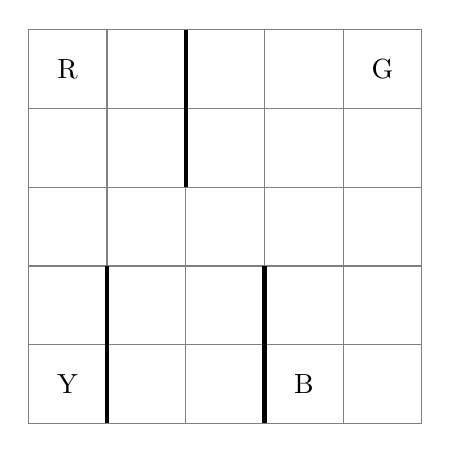
\begin{tikzpicture}
    % Grid
    \draw[step=1,color=gray] (0,0) grid (5,5);
    
    % Walls
    \draw[line width=1.5pt] (2,5) -- (2,3);
    \draw[line width=1.5pt] (1,0) -- (1,2);
    \draw[line width=1.5pt] (3,0) -- (3,2);

    % Pads
    \draw (0.5,4.5) node {R};
    \draw (0.5,0.5) node {Y};
    \draw (3.5,0.5) node {B};
    \draw (4.5,4.5) node {G};
\end{tikzpicture}
\end{document}

      \label{fig:taxi-domain}
    }
    \subfigure{
      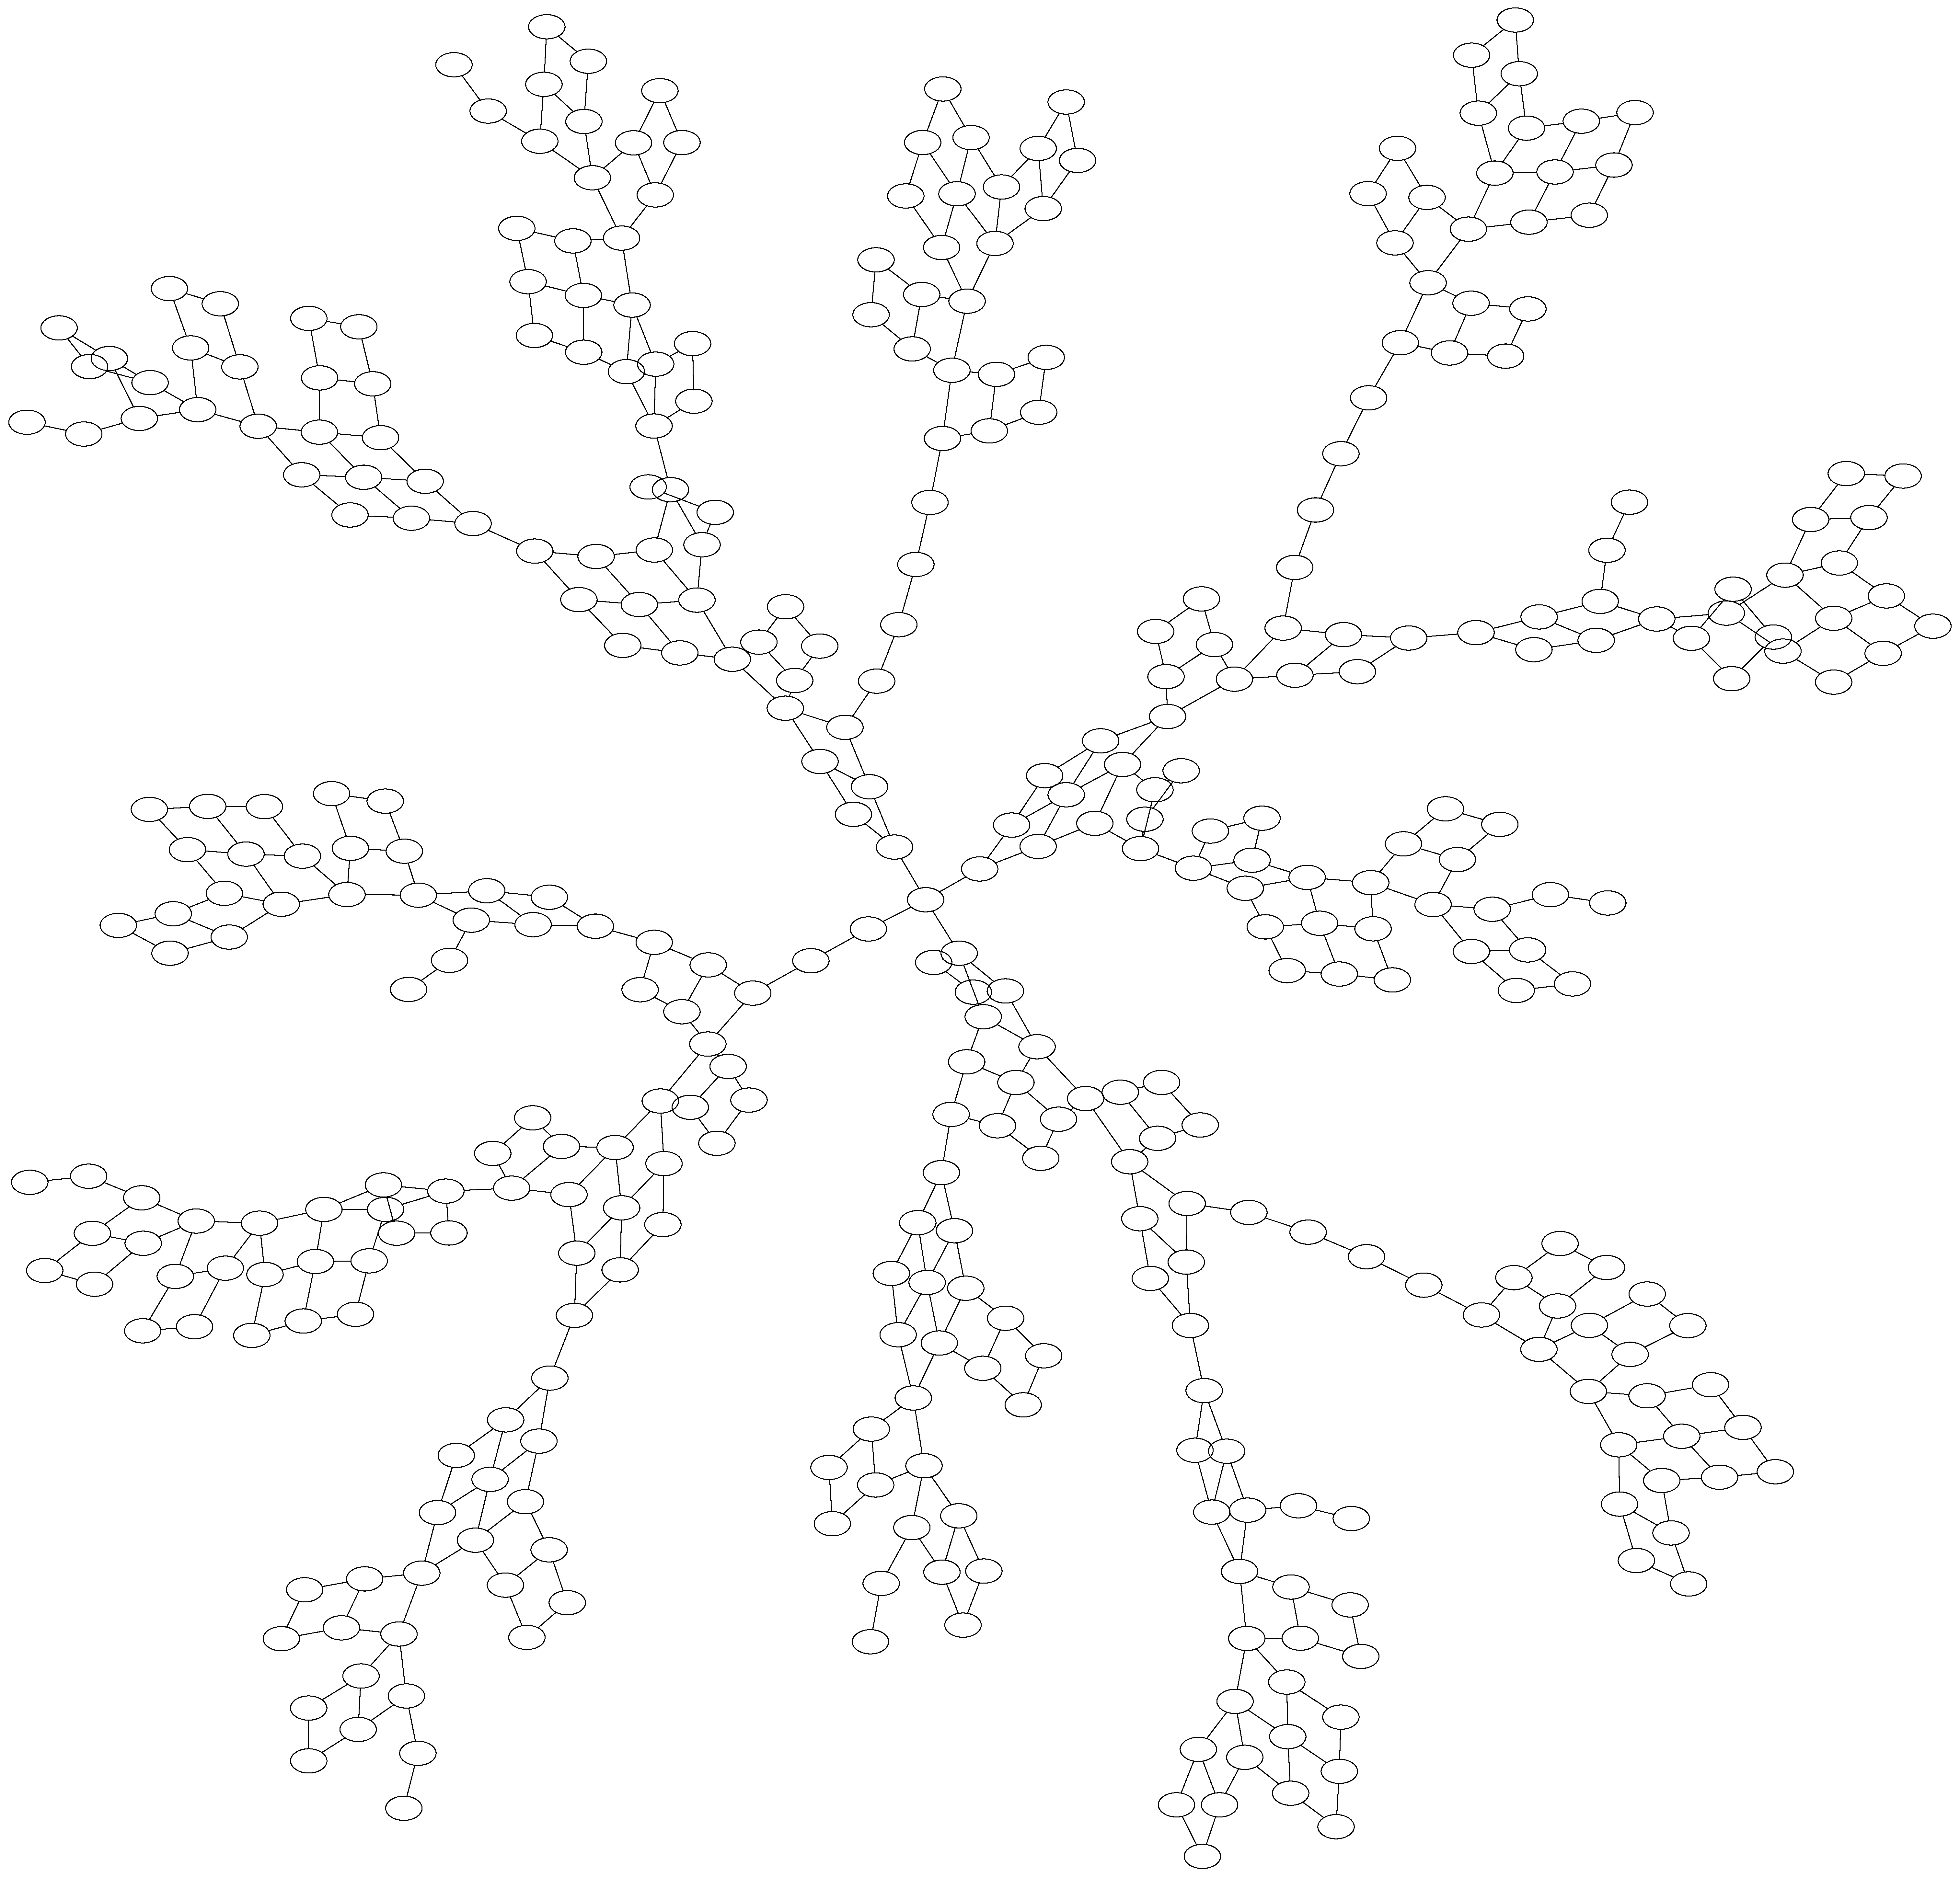
\includegraphics[height=2in]{figures/taxi1}
      \label{fig:taxi-graph}
    }
    \caption{The Taxi Domain, and its State Space Graph}
\end{figure*}

\begin{example}
  \label{example:taxi}
To make the discussion more tangible, let us look at an example, the
Taxi domain, shown in \figref{fig:taxi-domain}. The agent is a taxi
navigating in this road-map. It must pick up a passenger at one of the
4 pads, A, B, C or D.  Subsequently, it must carry the passenger to a
destination, which is also one of the above four pads. The states of
the taxi would then be a tuple containing the location of the
passenger (in one of the four pads, or within the taxi), the
destination of the passenger, and location of the taxi in the map.
The actions the taxi can perform are moving up, down, left or right in
the map, as well as pick up or drop a passenger at a pad. 
Typical options for such a domain would be an option that can be
started anywhere, and has a policy that takes the taxi to the one of
the pads in the shortest possible manner. Such an option is generic,
and does not depend on where the passenger or destination are. The RL
agent must then learn to choose the right option when picking up the
passenger.
\end{example}


% What are useful options? Highlight connection to connectivity, and
% then to small world options
\section{What are Useful Options?}
\label{sec:useful-options}

In this section, we will attempt to build a characterisation of what a
useful option is.

% Constructing Options 
We construct an option `short-circuiting' two states using a policy constructed
from the shortest path on this graph. For every state $x$, we select a state to
be short-circuited $y$ with using a multinomial distribution with weight
proportional to the distance between them in the state space, i.e. $w(x,y)
\propto d(x,y)^{-r}$. 

Another example of constructing an option on this graph would be to define a
policy that takes any state to a particular one along the shortest path. This is
the approach adopted by Simsek and Barto in \cite{Simsek}, where local maxima of
the betweenness scores are used to identify bottlenecks, and options defined to
reach these bottlenecks optimally from any state.




% Prove the interesting result
%\section{Approach}
\label{sec:approach}

% Explain small world
To answer this question, we look at the analysis of the ``small world
phenomenon'' in social networks by Kleinberg. Kleinberg defines the phenomenon
to be exhibited when when individuals can {\em efficiently} transmit a message
from source to destination knowing only the locations of their immediate
acquaintances with a decentralised algorithm. 
% Statement of Kleinberg's results
Consider a $k$-dimensional lattice of $n$ people \footnote{ Kleinberg's proofs
were limited to the $2$-dimensional case. Martel and Nyugen \cite{Martel2004}
extended them to the $k$-dimensional case }, wherein each person is connected to
one other person outside his/her immediate neighbours, according to the
distribution $P_{r}( u, v ) \propto \dist(u,v)^{-r}$, where $\dist(u,v)$
is the lattice distance between nodes $u$ and $v$, and $r$ is a parameter.
Kleinberg proves (a) that when $r=0$, i.e. the extra connections are uniformly
distributed, any decentralized algorithm will have an expected delivery time
that is exponential in $\tilde{d}$ (the shortest path length between $u$ and
$v$), and (b) when $r=k$, an algorithm can be constructed whose expected
delivery time is only polynomial of small degree in $\tilde{d}$.

Similarly, we define an MDP with options to exhibit the small world property
when an agent can efficiently reach a state of {\em maximal value} using only
its' local information. Using a similarly constructed $k$-dimensional lattice
for $\states$, where two states are connected by primitive actions if they are
neighbours, and by an option with an optimal deterministic policy otherwise. By
relating the distance of two states in the state space, and the difference in
value of the two states, we are able to prove that the expected number of {\em
decisions} an agent will have to make to reach a maximal value state will be poly-logarithmic in
$|\states|$.

% Describe the algorithms to; a) generate small world options b)
% extract from learning episodes
\section{Constructing Options from Experience} 
\label{sec:algo}

We saw in the previous section that we needed to generate $O(n)$ number
of path options. The utility of this method would severly be in question
if there was no efficient way to generate these options.

We make the observation that while we need $O(|S|)$ options, the
objective of the options is to bring the agent exponentially closer to
the maximal value state. Thus, we should be able to get away with
cheaply learnt options.

\begin{figure*}[ttt!]
  \begin{minipage}[t]{.49\textwidth}
    \begin{algorithm}[H]
      \caption{Small World Options from Experience}
      \label{algo:small-world-experience}
      \begin{algorithmic}[1]
          \REQUIRE $\mdp$, $\Rewards$, $r$, $n$, epochs, tasks
          \STATE $O \gets \emptyset$
          \FOR{ $i= 0 \to \textrm{tasks}$ }
            \STATE $\rewards \sim \Rewards$
            \STATE $Q \gets $ Solve $\mdp$ with $\rewards$ using
                $\frac{\textrm{epochs}}{\textrm{tasks}}$ epochs
            \STATE $O' \gets $ QOptions( $Q$, $r$,
                $\frac{n}{\textrm{tasks}}$ )
            \STATE $O \gets O \cup O'$
          \ENDFOR
          \RETURN A random subset of $n$ options from $O$
      \end{algorithmic}
    \end{algorithm}
  \end{minipage}
  \hfill
  \begin{minipage}[t]{.49\textwidth}
    \begin{algorithm}[H]
      \caption{{\bf QOptions}: Options from a $Q$-Value Function}
      \label{algo:qoptions}
      \begin{algorithmic}[1]
          \REQUIRE $Q$, $r$, $n$
          \STATE $O \gets \emptyset$
          \STATE $\pi \gets $ greedy policy from $Q$
          \FORALL{ $s$ in $\states$ }
            \STATE Choose an $s'$ according to $P_r$
            \IF{ $Q(s', \pi(s')) > Q(s, \pi(s))$ }
              \STATE $O \gets O \cup \tuple{\{s\}, \pi, \{s'\} \cup \{t \mid Q(s',\pi(s')) < Q(t, \pi(t))\} }$
            \ENDIF
          \ENDFOR{ $s$ in $\states$ }
          \RETURN A random subset of $n$ options from $O$
      \end{algorithmic}
    \end{algorithm}

  \end{minipage}
  \hfill
\end{figure*} 




% Experiment section
\section{Experimental Results}
\label{sec:experiments}
% Experimental results

We trained MacroQ learning agents on several standard domains, and
measured the cumulative return obtained using the following option
generation schemes: 
\begin{itemize}
   \item \textbf{None}: No options were used.
   \item \textbf{Random}: Options were generated by randomly connecting
     two nodes in the domain (this is equivalent to $P_0$.
   \item \textbf{Betweenness}: As a representative of bottleneck-based
     schemes, options were generated to take any node to a local maxima
     of betweenness centrality, as described in \cite{Simsek2008}. 
   \item \textbf{Small World}: Options were generated randomly
     connecting two nodes of the domain using an inverse square law, as
     described in \secref{sec:theory}.
\end{itemize}

Each experiment, unless mentioned otherwise, was run for $10$ randomly
generated tasks in the domain; each task ran for $40,000$ epochs, and
was averaged over an ensemble of $20$ agents.

\subsection{Optimal Options}
The agents were run on the following three domains using the algorithm
sketched in \secref{sec:theory}:
\begin{itemize}
   \item \textbf{Arbitrary Navigation}: The agent must reach an
     arbitrary goal state in an obstacle-free $x \times y$ grid-world. 
   \item \textbf{Rooms}: The agent must navigate a floor plan with
     4 rooms to reach an arbitrary goal state.
   \item \textbf{Taxi}: This is the domain described in
     \exref{example:taxi}.
\end{itemize}

The results of these experiments are summarised in
\autoref{tbl:optimal-returns}. Small world options perform significantly
better than the other schemes in navigation-oriented tasks like Rooms or
Arbitrary Navigation. In the Taxi domain, options generated by the
betweenness scheme outperform the small world options. This is expected
because the goal states in this domain lie at betweenness maxima.

\begin{figure*}[th]
    \center
    \subfigure[Options Learnt]{
      \includegraphics[height=2in]{figures/rooms-options}
      \label{fig:rooms-options}
    }
    \subfigure[Cumulative Return (with 200 options)]{
      \includegraphics[height=2in]{figures/rooms-return-200}
      \label{fig:rooms-return}
    }
    \caption{The Rooms Domain}
\end{figure*}

Some of the small world options preferred in Rooms domain are shown in
\figref{fig:rooms-options}. The graph shows several examples of options
that compose together to arrive near the goal state. We have also
plotted the learning behaviour in \figref{fig:rooms-return}. 

\begin{figure*}[th]
    \center
    \subfigure[$k$ vs Cumulative Return]{
      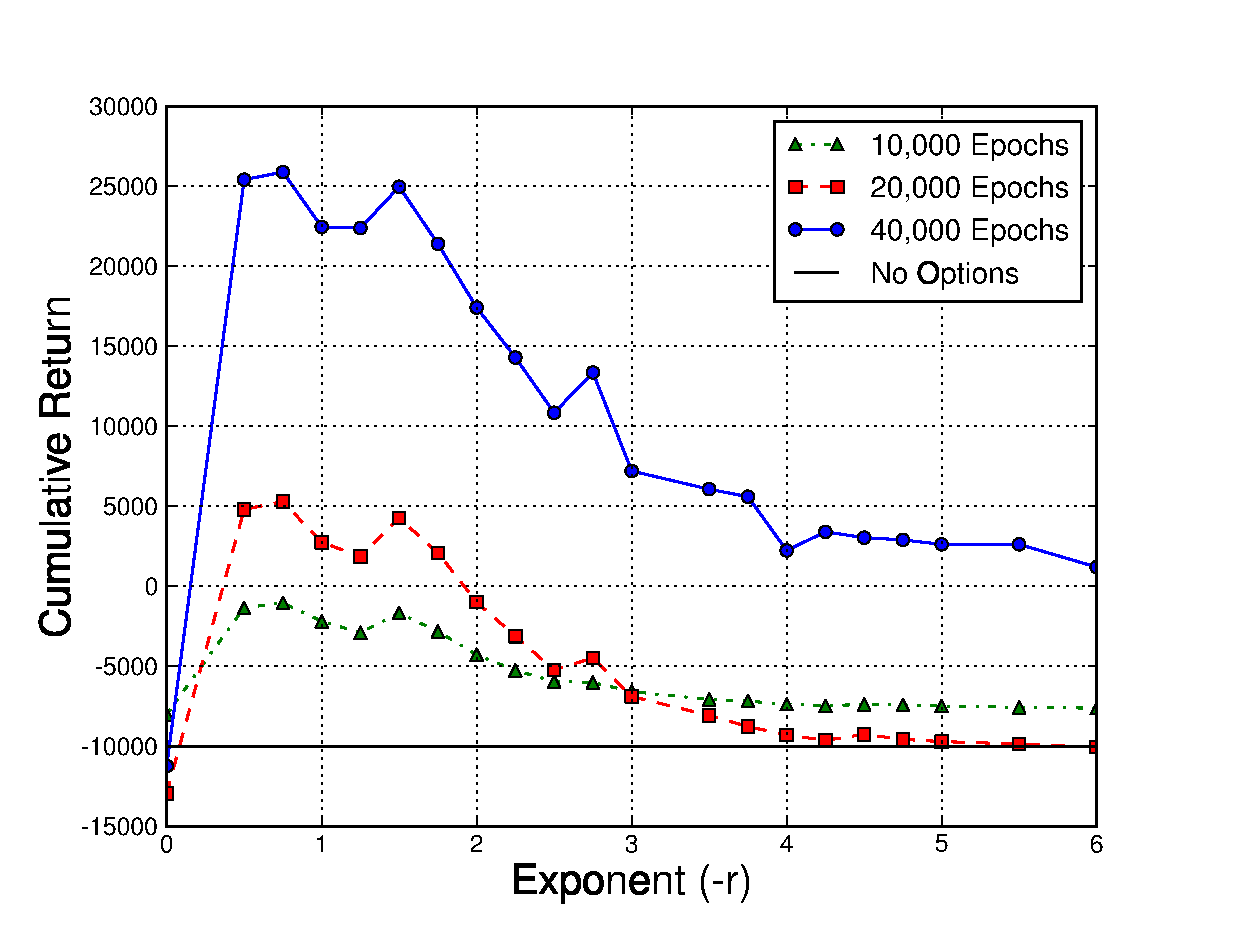
\includegraphics[height=2in]{figures/rooms-exp}
      \label{fig:rooms-exp}
    }
    \subfigure[Options Learnt on a Budget]{
    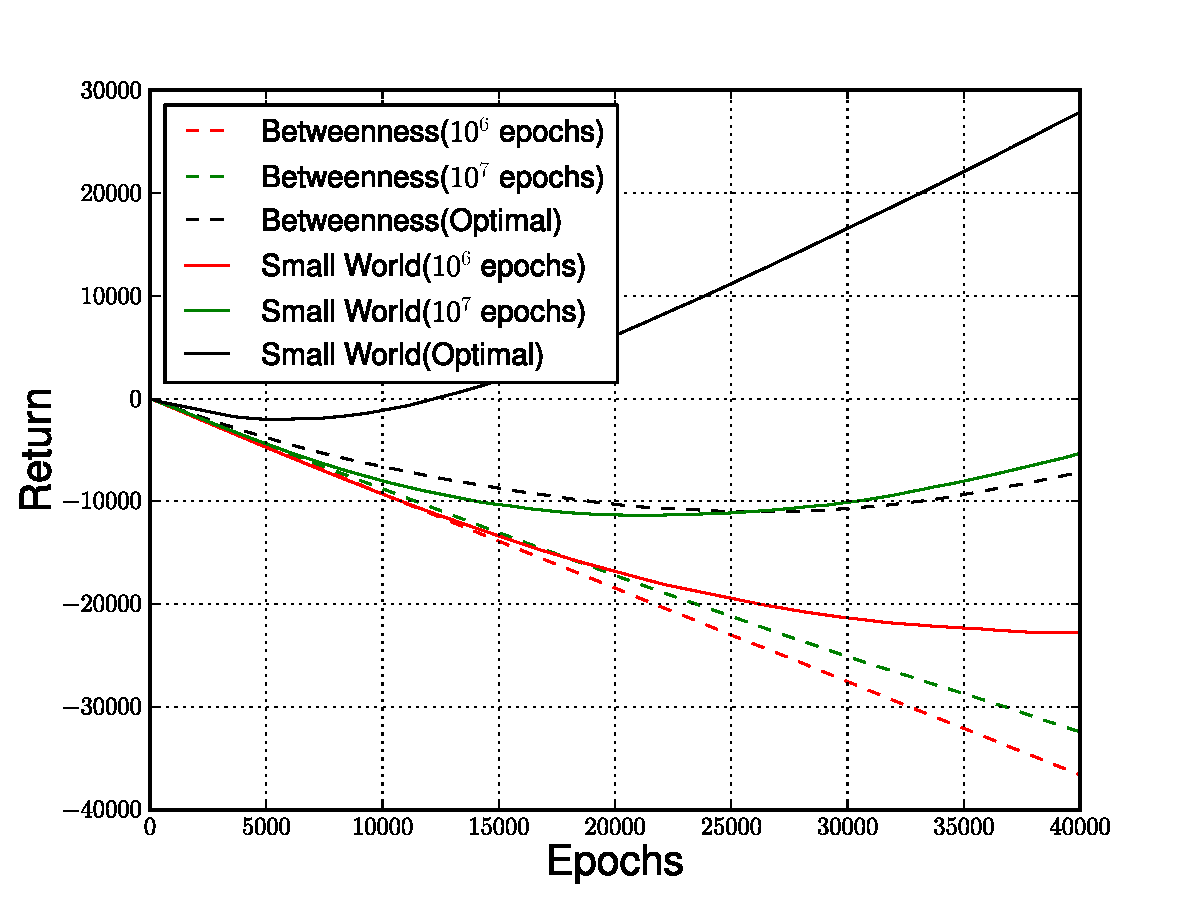
\includegraphics[height=2in]{figures/rooms-learnt-200}
      \label{fig:rooms-learnt}
    }
    \caption{The Rooms Domain (contd.)}
\end{figure*}

\subsection{Effect of $k$}
We do not yet have a clear understanding of how the exponent $k$ should
be chosen. \figref{fig:rooms-exp} plots $k$ versus the cumulative return
on the Rooms domain. The performance of the agent without options after
$20,000$ epochs is also plotted for reference. There is a range of $k$
($\approx 0.75$ to $1.5$) with good performance, after which the
performance steadily drops. This behaviour is easily explained; as the
exponent goes up, the small world options generated are very short, and
do not help the agent get nearer to the maximal value state. The optimal
range of $k$ is slightly counter-intuitive because the Rooms domain is
a two dimensional lattice with some edges removed. As a consequence of
the reduced connectivity, and perhaps due to stochastic factors, longer
range options are preferred.

\subsection{Options Learnt on a Budget}
In \secref{sec:algo}, we describe an algorithm to construct small world
options efficiently when given a limited number of learning epochs. We
compared the performance of these options with betweenness options
learnt similarly, and have plotted our results in
\figref{fig:rooms-learnt}. Despite using many more
options, the small world options thus created significantly outperform
betweenness options learnt with the same budget, and are even comparable
to the optimal betweenness options.


% Discuss conclusions
\section{Conclusions and Future Work}
\label{sec:conclusions}

% Contributions
% - new scheme for generating options
We have devised a new scheme to generate options based on small world
network model. The options generated satisfy an intuitive criteria, that
the subtasks learnt should be easily composed to solve any other task.
The options also greatly improve the connectivity properties of the
domain.

% - absolutely model-free
Experiments run on standard domains show significantly faster learning
rates using small world options. At the same time, we have shown that
learning small world options can be significantly cheaper than learning
`bottleneck' options. Another advantage of the scheme is that is does
not ever require the model of the MDP. We find it remarkable that we can
learn near optimal behaviour just from the policies of on some tasks


% - theoretical interest
The scheme does not perform any global analysis, and does not require
the model. We have shown that sample-wise, it can be far cheaper than
other bottleneck based methods. Does not lead to state space blow up.
Also is interesting from a theoretical perspective, logarithmic number
of decisions.

% Further work
% - dynamically add/remove options
% - figuring out r
We have as yet not been able to characterise what the exponent $r$
should be in a general domain. Given the ease with which options can be
discovered, it would be interesting to create a dynamic scheme.



\bibliographystyle{abbrv}
\bibliography{ref}{}

%\balancecolumns

\appendix
\section{Small Worlds}
\label{sec:small-worlds}

% Introduction and motivation for the proof
In this section, we will prove that the number of decisions taken by
an $\epsilon$-greedy agent, $\egreedyalgo$, to reach a maximal value
state in a $k$-dimensional lattice $\graph_k(V,E)$ is $O( (\log
V)^2)$. This is a simple extension to the Kleinberg's result. Our
approach is similar to that of Kleinberg's \cite{Kleinberg}, though we
adopt the somewhat cleaner notation of \cite{Martel2004}.

% Abstract result
Consider a $k$-dimensional lattice $\graph_k(V,E)$ with random links distributed
according to an inverse power law distribution $p(u,v) \propto \|u-v\|^{-k}$,
where $\|u - v\|$ is the distance between $u$ and $v$ in $\graph$. 

\begin{definition}
Let us define $\ball_l(u)$ to be the set of nodes contained within a
``ball'' of radius $l$ centered at $u$, i.e.  $\ball_l(u) = \{ v \mid
\|u - v\| < l \}$, and $\sball_l(u)$ to be the set of nodes on its
surface, i.e. $\sball_l(u) = \{ v \mid \|u - v\| = l \}$.
\end{definition}

We begin by finding the normalisation constant for the probability
distribution $p(u,v)$.

\begin{lemma}
    The inverse normalised coefficient for $p(u,v)$ is $c_u = \theta(
    \log n )$, and $p(u,v) = \|u - v\|^{-k} \theta( (\log n)^{-1} )$.
\end{lemma}
\begin{proof}
    \begin{eqnarray*}
        c_u &=& \sum_{v \ne u} \|u - v\|^{-k} \\
            &=& \sum_{j=1}^{k(n-1)} \sball_j(u) j^{-k}.
    \end{eqnarray*}
    It can easily be shown that the $\sball_l(u) = \theta( l^{k-1} )$.
    Thus, the $c_u$ reduces to a harmonic sum, and hence, $c_u =
    \theta( \log n )$.  The second part of the lemma follows as
    $p(u,v) = \frac{ \|u - v\|^{-k} }{c_u}$. 
    \\ \qed
\end{proof}

Now, consider a function $f$ embedded on $\graph(V,E)$, i.e. $f : V
\to \Re$, with the property that $\kappa_1 \|u-v\| - c_1 \le \|f(u) -
f(v)\| \le \kappa_2 \|u - v\| - c_2$, where $0 \le \kappa_1 \le
\kappa_2$, and $0 \le c_2 \le \frac{c_1}{2}$. Equivalently,
$\frac{\|f(u)-f(v)\| + c_2}{\kappa_2} \le \|u - v\| \le
\frac{\|f(u)-f(v)\| + c_1}{\kappa_1}$. We analogously define
$\ballf_l(u) = \{ v \mid \|f(u) - f(v)\| < l \}$. Let $M_f$ be the
global maxima of $f$. For notational convenience, we take $\ballf_l$
to be $\ballf_l(M_f)$.

% Describe problem / algo
\begin{definition}
    Let $\egreedyalgo$ be an $\epsilon$-greedy algorithm. If $N(u)$ is
    the next node chosen by $\egreedyalgo$, then $\egreedyalgo$
    chooses with probability $1-\epsilon$, the edge $(u,v)$ such that
    the distance of $v$ from the global maxima is minimum, i.e. $N(u)
    = \argmin_v \|v - f(M_f)\|$.
\end{definition}

We are now ready to prove the following general result.

\begin{theorem}
    \label{thm:decisions}
    \egreedyalgo takes $O( (\log n)^2 )$ decisions.
\end{theorem}
\begin{proof}
    Let a node $u$ be in phase $j$ when $u \in \ballf_{2^{j+1}}
    \setminus \ballf_{2^{j}}$. The probability that phase $j$
    will end this step is equal to the probability that $N(u) \in
    \ballf_{2^{j}}$. 
    
    The size of $\ballf_{2^{j}}$ is at least $|\ball_{\kappa_2^{-1}(
    2^{j}+c_2)}| = \theta( \kappa_2^{-k} (2^{j}+c_2)^{k} )$. The
    distance between $u$ and a node in $\ballf_{2^{j}}$ is at most
    $\frac{2^{j+1} + c_1}{ \kappa_1 } + \frac{2^{j} + c_2}{\kappa_2} <
    2(\frac{2^{j+1} + c_2}{\kappa_2})$. The probability of a link
    between these two nodes is at least $\kappa_1^{-k} (2^{j+2} + 2
    c_1)^{-k} \theta(\log n)^{-1} $. Thus, 

    \begin{eqnarray*}
        P(u, \ballf_{2^{j}} ) &\ge& (1-\epsilon) (\frac{2^{j}+c_2}{\kappa_2})^{k} \times (\frac{2^{j+2} + 2 c_1}{\kappa_1})^{-k} \theta( \log n )^{-1}  \\
        &\ge& \frac{(1-\epsilon)}{\theta( \log n )} \times (\frac{\kappa_1}{4\kappa_2} )^{k} \times ( \frac{ 1 + \frac{c_2}{2^{j}} }{ 1 + \frac{c_1}{2 \times 2^{j}} })^{k}\\
        &\ge& \frac{(1-\epsilon)}{\theta( \log n )} \times (\frac{\kappa_1}{4\kappa_2} )^{k} \times ( \frac{ 1 + c_2 }{ 1 + \frac{c_1}{2} })^{k} .\\
    \end{eqnarray*}

    Let number of decisions required to leave phase $j$ be $X_j$. Then, 
    \begin{eqnarray*}
        \E[X_j] &\le& \sum_{i=0}^{\infty} (1 - P(u, \ballf_{2^{j}} ))^i \\
                &\le& \frac{1}{P(u, \ballf_{2^{j}} )} \\
                &\le& \theta( \log n ) \frac{1}{(1-\epsilon)} (\frac{4 \kappa_2}{\kappa_1})^{k} ( \frac{ 1 + \frac{c_1}{2} }{ 1 + c_2 })^{k}\\
                &\le& \theta( \log n ).
    \end{eqnarray*}
    Thus, $\E[X_j]$ is $O(\log n)$. By construction, there are at most $\log n$
    phases, and thus at most $O((\log n)^2)$ decisions.
    \\ \qed
\end{proof}


%\balancecolumns 

\end{document}

